\documentclass[a4paper,twoside,12pt]{report}
% Richard Klein (2020,2021)

% Include Packages
%\usepackage[a4paper,inner=3.5cm,outer=2.5cm,top=2.5cm,bottom=2.5cm]{geometry}  % Set page margins
\usepackage{fullpage}
\usepackage{float}                  % Allows 'Here and Only Here' [H] for Floats
\usepackage{url}                    % \url{} command
\usepackage{charter}                  % Set font to Times
\usepackage{graphicx}               % \includegraphics
\usepackage{subfigure}              % Allow subfigures
\usepackage{amsmath}
\usepackage{amssymb}
\usepackage{amsthm}
\usepackage{booktabs}
\usepackage{parskip}
\usepackage[all]{nowidow}
\usepackage{pdflscape}
\usepackage{longtable}


\setnoclub[2]
\setnowidow[2]

% Referencing
% Provides \Vref and \vref to indicate where a reference is.
\usepackage{varioref} 
% Hyperlinks references
\usepackage[bookmarks=true,bookmarksopen=true]{hyperref} 
% Provides \Cref, \cref, \Vref, \vref to include the type of reference: fig/eqn/tbl
\usepackage{cleveref} 
% Setup Hyperref
\hypersetup{
  colorlinks   = true,              %Colours links instead of ugly boxes
  urlcolor     = blue,              %Colour for external hyperlinks
  linkcolor    = blue,              %Colour of internal links
  citecolor    = blue                %Colour of citations
}
% Names for Clever Ref
\crefname{table}{table}{tables}
\Crefname{table}{Table}{Tables}
\crefname{figure}{figure}{figures}
\Crefname{figure}{Figure}{Figures}
\crefname{equation}{equation}{equations}
\Crefname{equation}{Equation}{Equations}

% Wits Citation Style
\usepackage{natbib} \input{natbib-add}
\bibliographystyle{named-wits}
\bibpunct{[}{]}{;}{a}{}{}  % to get correct punctuation for bibliography
\setlength{\skip\footins}{1.5cm}
\newcommand{\citets}[1]{\citeauthor{#1}'s \citeyearpar{#1}}
\renewcommand\bibname{References}  

\pagestyle{headings}

\pagestyle{plain}
\pagenumbering{roman}

\renewenvironment{abstract}{\ \vfill\begin{center}\textbf{Abstract}\end{center}\addcontentsline{toc}{section}{Abstract}}{\vfill\vfill\newpage}
\newenvironment{declaration}{\ \vfill\begin{center}\textbf{Declaration}\end{center}\addcontentsline{toc}{section}{Declaration}}{\vfill\vfill\newpage}
\newenvironment{acknowledgements}{\ \vfill\begin{center}\textbf{Acknowledgements}\end{center}\addcontentsline{toc}{section}{Acknowledgements}}{\vfill\vfill\newpage}

\begin{document}
\onecolumn
\thispagestyle{empty}

\setcounter{page}{0}
\addcontentsline{toc}{chapter}{Preface}
\ 
\begin{center}
  \vfill
  {
  \huge \bf \textsc{The Development of Cyber Threat Intelligence System Framework for the Mining Industry}\\
  \rule{\linewidth}{0.5pt}

%   \large Subtitle\\[20pt]


  \normalsize
  Proposed by:\\
  MUHAMMAD UMER FAROOQ\\
  2925331\\[20pt]
  Supervisors:\\[10pt]
  Dr. Helen Robertson\\[10pt]
  Dr. Ahsan Mahboob\\[10pt]
  \today
  }
  \vfill

  \vfill
  
\includegraphics[width=2.5cm]{images/wits.png}
  \vfill
  \vfill

%   \vspace{10pt}\\
  % \small{Ethics Clearance Number: XX/XX/XX}\\[10pt]
  \small{A proposal submitted to the Faculty of Science, University of the Witwatersrand, Johannesburg,
in partial fulfilment of the requirements for the degree of Master of Science (Dissertation) in Computer Science}\\
\rule{\linewidth}{0.5pt}
\large School of Computer Science \& Applied Mathematics\\
\large University of the Witwatersrand\\[20pt]

\end{center}
\vfill
\newpage

\pagestyle{plain}
\setcounter{page}{1}

\phantomsection
\begin{abstract}
The mining industry's growing reliance on digital technologies has significantly increased its vulnerability to cyber threats, which can lead to severe operational, financial, and environmental consequences. This research aims to develop a comprehensive Cyber Threat Intelligence (CTI) system tailored specifically for the mining sector, utilizing advanced data analytics and machine learning to enhance cyber threat detection and mitigation capabilities. A mixed-methods approach combining systematic literature reviews, empirical testing, and qualitative analyses ensures a robust framework that addresses both technical and ethical considerations. The proposed CTI system will gather, aggregate, and analyze data from diverse sources, such as network logs and open-source intelligence feeds, employing machine learning techniques to identify patterns and anomalies indicative of cyber threats. This research also critically examines the ethical implications of deploying such systems, ensuring compliance with industry standards and regulations. By integrating stakeholder feedback throughout the development and implementation phases, the study ensures that the CTI system is practical, effective, and aligned with the mining industry’s specific needs. The anticipated outcomes include improved resilience against cyber threats, minimized risk of operational disruptions, and enhanced protection of sensitive data and infrastructure. This research contributes to the broader field of cybersecurity in critical infrastructure, providing valuable insights into the application of CTI systems within industry-specific contexts.
\end{abstract}

\phantomsection
\begin{declaration}
I, Muhammad Umer Farooq, hereby declare the contents of this research proposal to be my own work.
This proposal is submitted for the Master of Science by Dissertation in Computer Science at the University of the Witwatersrand.
This work has not been submitted to any other university, or for any other degree.
\end{declaration}

\phantomsection
\begin{acknowledgements}
I would like to express my deepest gratitude to my supervisors, Dr. Helen Robertson from the School of Computer Science and Mathematics, and Dr. M. Ahsan Mahboob, the Head of Sibanye Stillwater Digital Mining Laboratory (DigiMine), for their invaluable guidance and support throughout my research journey. I would like to thank and acknowledge the financial support provided by the Sibanye-Stillwater Digital Mining Laboratory (DigiMine), Wits Mining Institute (WMI).

Dr. Robertson’s expertise and insightful feedback were instrumental in refining my work, and her encouragement was a constant source of motivation. I am equally grateful to Dr. Mahboob for his mentorship and for providing me with the opportunity to collaborate within the DigiMine lab, where his leadership and profound knowledge in the field greatly enhanced my research experience.

Their unwavering support, constructive feedback, and encouragement have been crucial to the successful completion of this proposal. I am deeply appreciative of their time and efforts, and I feel privileged to have worked under their guidance.
\end{acknowledgements}


\phantomsection
\addcontentsline{toc}{section}{Table of Contents}
\tableofcontents
\newpage
\phantomsection
\addcontentsline{toc}{section}{List of Figures}
\listoffigures
\newpage
\phantomsection
\addcontentsline{toc}{section}{List of Tables}
\listoftables
\newpage
\pagenumbering{arabic}
% Chapter 1
\chapter{Introduction}
The Mining Industry is as important part of the global economy. It depends on digital technologies to improve operations, safety, and sustainability. However, this reliance on technology exposes the industry to significant cyber threats that can disrupt operations, compromise safety, and cause financial loss and environmental harm. Given these risks, the need for effective cyber threat detection in mining is more urgent than ever. Traditional and reactive cybersecurity measures often fail to address the complex and evolving threats specific to the mining sector. This has led to the growing importance of Cyber Threat Intelligence (CTI) System for the mining sector, which proactively detect, analyze, and respond to potential threats using intelligence feeds. These systems collect and analyze data from multiple sources, helping organizations identify and mitigate risks before they cause damage. Despite potential threats, the urgency for effective cyber threat detection in mining has never been greater. Traditional reactive cybersecurity measures used in the sector often fall short of addressing the sophisticated and evolving threats unique to the mining sector. This research aims to fill these gaps by developping tailored Cyber Threat Intelligence System Framework specifically for the mining industry. The CTI Framework will use advanced data analytics and machine learning algorithms to detect patterns and anomalies in threats datam and it will improve the industry’s ability to defend against cyber-attacks. Additionally, this study will examine the ethical implications of implementing such a system, ensuring it meets both technical and ethical standards. By designing a CTI system tailored to the mining sector, this research will address a critical need and contribute to the broader field of cybersecurity. In Figure: \ref{fig:thing1}, World Economic Forum Global Risks Perception Survey 2023-2024 indicating a wide subset of the global population to potential digital and physical exploitation.

\begin{figure}[ht]
    \centering
    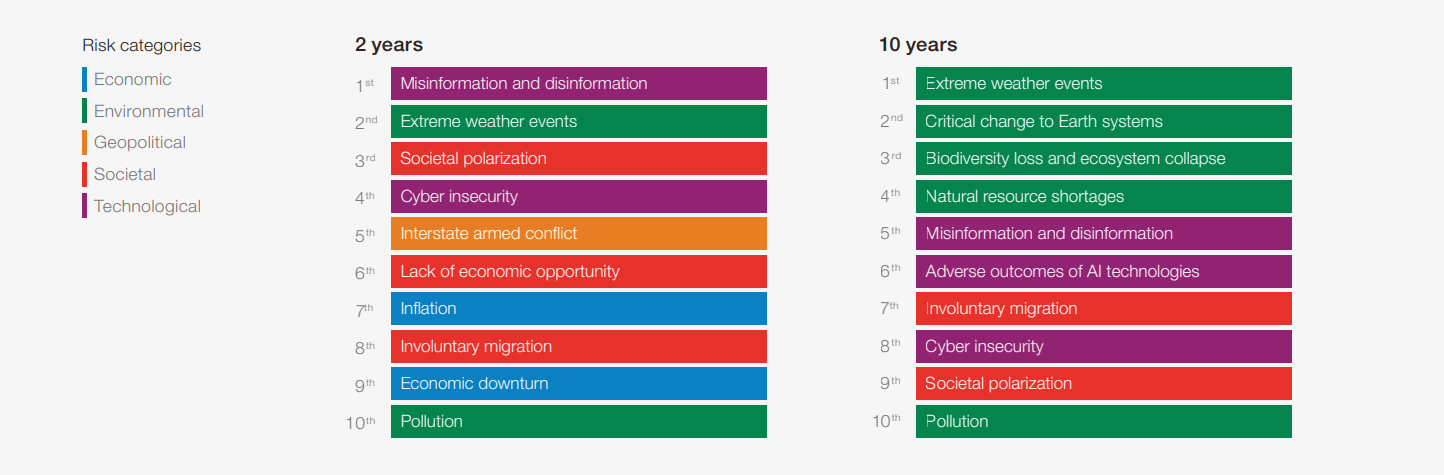
\includegraphics[width=1.0\linewidth]{images/world-economic-forum-global-risks.png}  % If located in the "images" folder
    \caption{World Economic Forum Global Risks Analysis Survey 2023-2024}
    \label{fig:thing1}
\end{figure}

\section{Problem Statement}
Mining Industry plays a crucial role in global economic development. Mining operations are adopting digital technologies rapidly to enhance productivity, safety, and efficiency. These are becoming more vulnerable to cyber threats. These threats can disrupt operations, can compromise sensitive data, can cause financial loss, and even it can endanger lives and the environment. Evolution Mining is an Australian gold mining company. It suffered a ransomware attack in August 2024 on its IT systems, which, though swiftly contained, underscored the industry's susceptibility to cyber threats. A month earlier, in July 2024, Sibanye-Stillwater also faced a cyberattack, leading to temporary IT system outages and manual processing in some of its operations. Norsk Hydro is a major metals and mining company. It experienced a ransomware attack in 2020 that caused significant operational shutdowns and millions in losses.
An attack on a South American in 2017 on a mining firm compromised sensitive geological data. An Australian mining company suffered unauthorized access in 2019 which disrupted automated processes and risked worker safety.
These incidents highlight the urgent necessity for robust, proactive cybersecurity measures to protect the industry from evolving threats.


% 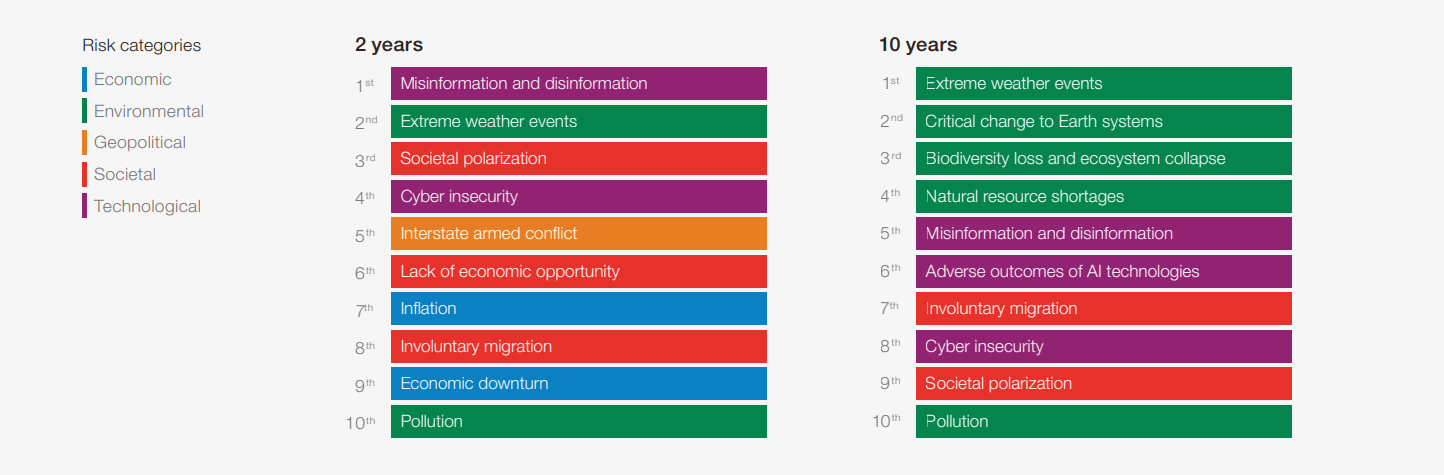
\includegraphics[width=1.0\linewidth]{images/world-economic-forum-global-risks.png}  % If located in the "images" folder
% \caption{World Economic Forum Global Risks Perception Survey 2023-2024}



\section{Research Questions}
% \section{Research Questions}

The following questions are formulated to guide the research for development of a Cyber Threat Intelligence (CTI) system tailored for the mining industry:

\begin{enumerate}
    \item {How can a framework for a Cyber Threat Intelligence (CTI) system be developed specifically for the mining industry?}
 \item {What strategies and technologies can be utilized to efficiently collect, aggregate, and analyze cyber threat data from sources like network logs and open-source intelligence feeds for the mining industry?}

    \item {How can advanced data analysis and machine learning techniques be applied to detect and analyze patterns and anomalies in cyber threat data specific to the mining sector?}

    \item {What are the ethical challenges associated with implementing a CTI system in the mining industry, and how can these be effectively addressed to align with ethical standards and regulations?}
\end{enumerate}
\section{Research Aims and Objectives}
The adoption of digital technologies in the mining industry is essential for advancing productivity and safety. But it has also led it to significant cyber vulnerabilities. Cyber threats continuing to evolve. So, the need for a proactive approach to identify, analyze, and mitigate risks has become essential. The research aims and objectives focus on developing a robust CTI system Framework.\\
\subsection{Research Aims}
The primary aim of this research is to develop an effective Cyber Threat Intelligence (CTI) framework for the mining industry, designed to enhance cybersecurity resilience. This research aims to mitigate the increasing cyber threat risks within the mining industry, which has seen a sharp rise in digital vulnerabilities as it adopts more advanced technologies by developing a CTI Framework tailored to mining industry. This aim involves creating a specialized CTI system that can detect and respond to cyber threats, ensuring the safety, security, and continuity of mining operations in an increasingly digitalized environment.
\subsection{Research Objectives}

The objectives of this research are as follows:

\begin{itemize}
    \item Develop a framework for a Cyber Threat Intelligence (CTI) System tailored specifically to the mining industry.
    \item To collect, aggregate, and analyze threat data from various sources, including network logs and open-source intelligence feeds.
    \item To apply advanced data analysis and machine learning techniques to identify patterns and anomalies within the collected threat data.
    \item To examine and address the ethical considerations and implications of implementing a CTI framework within the mining industry.
\end{itemize}
\section{Limitations}
The basic limitation of this research is the generalizability of its findings across the diverse operational environments within the mining industry. While the study aims to develop a robust Cyber Threat Intelligence (CTI) Framework tailored to mining, it relies on specific datasets and threat scenarios that may not comprehensively reflect all real-world contexts. Differences in mining operations, network architectures, and data characteristics across various geographical and organizational settings could impact the performance and applicability of the CTI framework. Additionally, the effectiveness of the proposed data analysis and machine learning techniques in detecting threats and enhancing model interpretability may vary depending on the complexity and heterogeneity of cyber threat data across mining entities. Consequently, while the research aspires to make valuable contributions to the mining sector's cybersecurity capabilities, its application to the broader landscape of mining operations may be constrained.\\
\section{Overview}

The digital transformation of the mining industry has driven significant improvements in operational efficiency, safety, and environmental sustainability. Technologies such as IoT, data analytics, and automation have enhanced mining processes; however, they have also introduced new cybersecurity vulnerabilities. These digital advancements expose mining operations to sophisticated cyber threats, which can disrupt production, compromise sensitive data, lead to financial losses, and even endanger lives. Given the critical nature of mining infrastructure, a proactive approach to cybersecurity is essential to ensure both the safety and continuity of operations.

Traditional cybersecurity solutions are often inadequate to address the mining industry’s specific needs due to the unique operational environments, remote locations, and reliance on legacy systems. To address these gaps, this research proposes the development of a Cyber Threat Intelligence (CTI) framework designed specifically for the mining industry. This framework aims to leverage advanced data analytics and machine learning to detect, analyze, and respond to cyber threats more effectively, thereby increasing the industry’s resilience against evolving cyber risks.

The proposed CTI framework will aggregate data from diverse sources, including network logs and open-source intelligence feeds, to detect patterns and anomalies indicative of cyber threats. The framework is structured to support real-time monitoring and rapid response, tailored to the operational and technical requirements of the mining sector. Additionally, this study will examine the ethical considerations associated with implementing such a system, ensuring compliance with industry standards and regulations to protect privacy and uphold data integrity.

By developing a CTI framework specific to the mining industry, this research intends to provide a robust solution for safeguarding critical mining infrastructure. The anticipated outcomes include enhanced threat detection capabilities, reduced risk of operational disruptions, and improved protection of sensitive data and resources. This research not only contributes to the cybersecurity of the mining industry but also offers insights into the application of CTI systems in other critical infrastructure sectors facing similar digitalization challenges.



% \subsubsection{This is a subsubsection}
% This is just a paragraph
% \subsection{A Subsection about Citation Style}
% Citations are important. Citation style for Computer Science is:
% \begin{itemize}
% \item When used in the text, use the authors with the date in brackets:\\ \citet{klein17} say very important things.
% \item When used as a reference after a face, put everything in brackets:\\ Import things are true \citep{klein17}.
% \end{itemize}

% \subsection{Compiling}
% Remember to compile multiple times to resolve references. Usually:
% \begin{verbatim}
% pdflatex file.tex
% bibtex file
% pdflatex file.tex
% pdflatex file.tex
% \end{verbatim}

% Chapter 2
\chapter{Background and Literature Review}

\section{Introduction}
This chapter discusses the background and prior research related to Cyber Threat Intelligence (CTI) systems in detail. This section provides the foundational understanding of CTI frameworks and situates the current research within the context of existing literature. The review covers the evolution of cybersecurity challenges in the mining industry, key components of CTI frameworks, and the use of data analytics and machine learning techniques to identify cyber threats. The chapter also discusses the ethical considerations and regulatory requirements relevant to developing a CTI system in a highly specialized industrial environment.

\section{Background}
The mining industry's integration into the digital ecosystem has resulted in increased automation, improved safety measures, and enhanced operational efficiency. However, this dependence on digital technology has simultaneously made mining operations susceptible to sophisticated cyber threats. These threats are often complex, ranging from ransomware attacks that can halt operations to Advanced Persistent Threats (APTs) aimed at stealing valuable intellectual property.

\subsection*{Industry 4.0 and Digitalization}
The concept of Industry 4.0 has brought a digital transformation across sectors, including mining, through the use of IoT, machine learning, cloud computing, and big data. In mining, technologies like real-time monitoring systems, autonomous mining equipment, and predictive maintenance are becoming the norm. However, this transformation exposes critical infrastructure to cyber vulnerabilities \citep{wang2013cyber, sajid2016cloud}.

\subsection*{Cyber Threat Landscape in Mining}
The mining sector faces unique cyber threats due to the critical nature of its operations. Examples of past cyber incidents include ransomware attacks and data breaches targeting geological data or disrupting automated processes. High-profile cases like the ransomware attack on Evolution Mining in 2024 and Norsk Hydro's incident in 2020 illustrate the potential impact on productivity and financial stability.

\subsection*{SCADA Systems and Vulnerabilities}
Supervisory Control and Data Acquisition (SCADA) systems are widely used in mining to monitor and control physical processes. However, traditional SCADA systems lack the security measures necessary to counter the vulnerabilities introduced by cloud and IoT integrations. The need for an advanced CTI system becomes evident, as these vulnerabilities can lead to catastrophic failures in mining operations \citep{wang2013cyber}.

\subsection*{Cybersecurity Challenges Unique to Mining Operations}
\begin{itemize}
    \item \textbf{Remote and Harsh Environments:} Mining operations are often located in remote areas with limited connectivity, making it challenging to deploy and maintain comprehensive cybersecurity solutions.
    \item \textbf{Legacy Systems and Modernization:} Many mining facilities still use outdated systems that are difficult to secure, and updating these without causing operational disruptions is a significant challenge.
    \item \textbf{Supply Chain Vulnerabilities:} The mining industry relies heavily on third-party vendors and contractors, which introduces additional security risks and necessitates robust supply chain security measures.
\end{itemize}

\section{Related Work}
\subsection{Cyber Threat Intelligence (CTI) Frameworks}
CTI frameworks have emerged as crucial solutions for enhancing the proactive capabilities of cybersecurity defenses. They leverage data collection, analysis, and dissemination to provide actionable insights into emerging threats. Various researchers have proposed different components for CTI frameworks, each tailored to address specific cybersecurity needs.


\subsubsection*{Existing Framework Comparison}
Existing Cyber Threat Intelligence (CTI) frameworks vary in structure, focus, and capabilities, addressing different facets of cybersecurity needs across industries. A comparison of prominent CTI frameworks reveals a variety of approaches to data collection, analysis, and intelligence dissemination, which contribute uniquely to threat intelligence development.

\paragraph{MITRE ATT\&CK Framework \citet{georgiadou2021assessing}}
\textit{Focus:} Threat tactics, techniques, and procedures (TTPs) \citet{shahi2018tactics}. \\
\textit{Components:} Provides a detailed matrix of attack techniques that allow organizations to understand the methods and behaviors of adversaries. \\
\textit{Adoption:} Widely adopted across multiple sectors, MITRE ATT\&CK assists in understanding attacker behavior and mapping defensive measures to specific threat actions.

\paragraph{Diamond Model of Intrusion Analysis \citet{caltagirone2013diamond}}
\textit{Focus:} Links threat activity to the context, including attacker, infrastructure, and victim relationships. \\
\textit{Components:} Emphasizes understanding the relationships between adversaries and their targets by examining the four core elements—adversary, infrastructure, capability, and victim. \\
\textit{Adoption:} Popular in critical infrastructure sectors, it aids in identifying threat campaigns and understanding complex threat vectors.

\paragraph{Lockheed Martin Cyber Kill Chain \citet{naik2022comparing}}
\textit{Focus:} The stages of cyber attacks, from initial intrusion to data exfiltration. \\
\textit{Components:} Includes stages like reconnaissance, weaponization, delivery, exploitation, and actions on objectives. \\
\textit{Adoption:} Utilized by security teams to map out attack stages and identify gaps in defenses for preemptive countermeasures.

\paragraph{STIX/TAXII Protocols \citet{provatas2023standards}}
\textit{Focus:} Standardized threat data formatting and sharing. \\
\textit{Components:} Structured Threat Information Expression (STIX) provides a common language for sharing threat intelligence, while Trusted Automated Exchange of Indicator Information (TAXII) facilitates secure and automated data exchange. \\
\textit{Adoption:} Primarily used by organizations seeking interoperability in threat data sharing, enhancing collaboration across different cybersecurity platforms.

\paragraph{OpenIOC \citet{janotistrategic}}
\textit{Focus:} Rapid identification of indicators of compromise (IOCs). \\
\textit{Components:} Offers a framework for describing, archiving, and sharing threat intelligence specific to forensic artifacts and attack indicators. \\
\textit{Adoption:} Commonly used for incident response to detect and isolate threats based on predefined IOCs.

\subsubsection*{CTI Framework Adoption in Other Critical Infrastructures \citet{kayode2023applications}}
Cyber threat intelligence frameworks have been increasingly adopted across various critical infrastructure sectors, such as energy \citet{gong2021cyber}, healthcare, finance, and government, where cybersecurity is paramount to ensure continuity and protect against disruptive attacks.

\paragraph{Energy Sector \citet{gong2021cyber}}
\textit{Application:} The energy sector, particularly in Supervisory Control and Data Acquisition (SCADA) systems, uses frameworks like MITRE ATT\&CK and the Diamond Model to detect and respond to attacks that could affect power grid stability. \\
\textit{Challenges:} Due to the complexity and real-time nature of SCADA systems, CTI frameworks in this sector often incorporate advanced analytics and machine learning for anomaly detection to ensure rapid threat mitigation. \\
\textit{Examples:} Many energy companies have adopted the Cyber Kill Chain model to prevent and disrupt threats across the different stages of cyberattacks targeting power grids.

\paragraph{Healthcare Sector \citet{krauss2022analysis}}
\textit{Application:} CTI frameworks like STIX/TAXII are widely used in healthcare for secure threat intelligence sharing, especially for protecting patient data and healthcare services. \\
\textit{Challenges:} Healthcare networks, which contain sensitive patient information and are increasingly targeted by ransomware, rely on frameworks with strong data privacy and real-time response capabilities. \\
\textit{Examples:} Integration with ISACs \citet{bugiardini2016international} for the healthcare sector provides enhanced collaboration and intelligence sharing to keep up with rapid threat evolution.

\paragraph{Financial Sector \citet{bin2024maximizing}}
\textit{Application:} The financial industry uses frameworks like MITRE ATT\&CK to monitor and respond to fraud, phishing, and advanced persistent threats (APTs) targeting financial institutions. \\
\textit{Challenges:} Given the sector's high vulnerability to fraud and data theft, CTI frameworks are often tailored to identify threat vectors unique to financial data and transactions, such as money laundering and payment fraud. \\
\textit{Examples:} Financial institutions participate in FS-ISAC, a sector-specific information-sharing platform that allows them to stay ahead of cross-border cyber threats.

\paragraph{Government and Defense \citet{bin2024maximizing}}
\textit{Application:} Governments and defense sectors use comprehensive CTI frameworks like MITRE ATT\&CK and Diamond Model to protect national security infrastructure. \\
\textit{Challenges:} These sectors face complex threats from state-sponsored actors, necessitating robust intelligence sharing and high-level threat attribution capabilities. \\
\textit{Examples:} Government agencies often utilize frameworks integrated with global intelligence alliances and automated response systems to mitigate sophisticated attacks on critical infrastructure.

\subsubsection*{Components of a CTI Framework}
\paragraph{CTI Data Collector}
\textit{Role and Functionality:} The data collector component is responsible for aggregating raw cyber threat data from multiple sources. These include OSINT feeds, network logs, vendor-provided threat intelligence, and even data from the dark web. The data collected must be diverse and comprehensive to ensure accurate threat detection.

\textit{Literature Examples:}
\begin{itemize}
    \item \citep{lee2016open}: Developed an OSINT-focused data collection strategy that ensures timely and relevant threat information. Their framework emphasizes preparing and implementing an OSINT plan before gathering and analyzing data from open sources. In Fig.~\ref{fig:thing1}, we see the OSINT-based Cyber Threat Inspection Framework proposed by \cite{lee2016open}, designed specifically for critical infrastructures.
    \begin{figure}[ht]
        \centering
        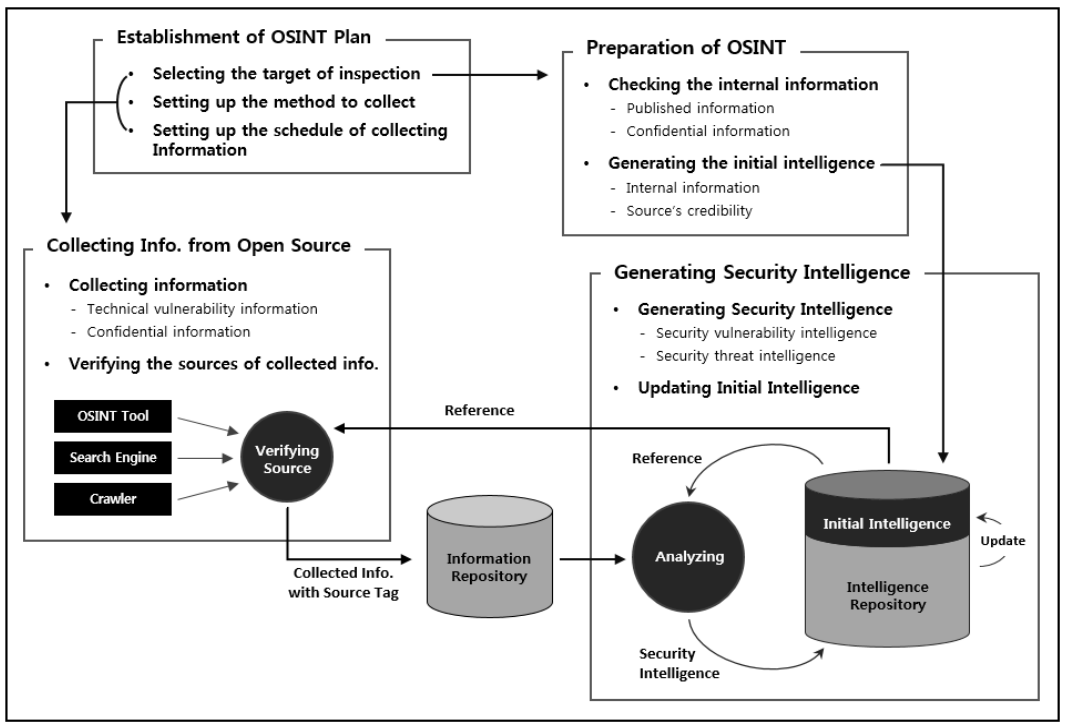
\includegraphics[width=1.0\linewidth]{images/osint-based-cti-framwork.png}  % If located in the "images" folder
        \caption{\citep{lee2016open} proposed Open Source Intelligence base Cyber Threat Inspection Framework for Critical Infrastructures}
        \label{fig:thing1}
    \end{figure}
    \item \citep{ryandy2020xt}: Outlined a systematic approach to data collection, emphasizing the importance of processing, analysis, and evaluation to ensure that the collected data is usable for threat intelligence purposes.
    \begin{figure}[ht]
        \centering
        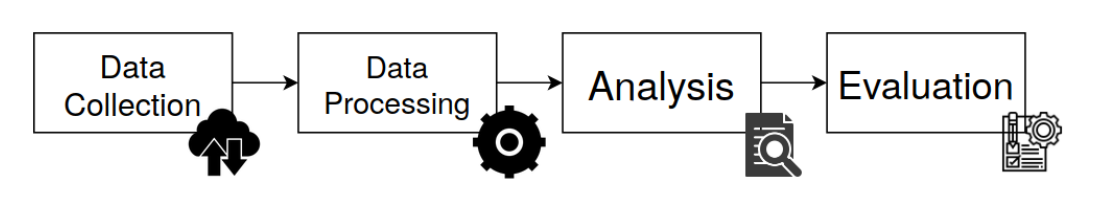
\includegraphics[width=1.0\linewidth]{images/data-collection-for-osint.png}  % If located in the "images" folder
        \caption{Research Framework for Data Collection proposed by \citep{ryandy2020xt}}
        \label{fig:thing1}
    \end{figure}
    \item \citep{tundis2022feature}: Focused on feature selection and OSINT source identification, demonstrating that a well-designed data collection system can significantly impact the quality of threat intelligence.
    \begin{figure}[ht]
        \centering
        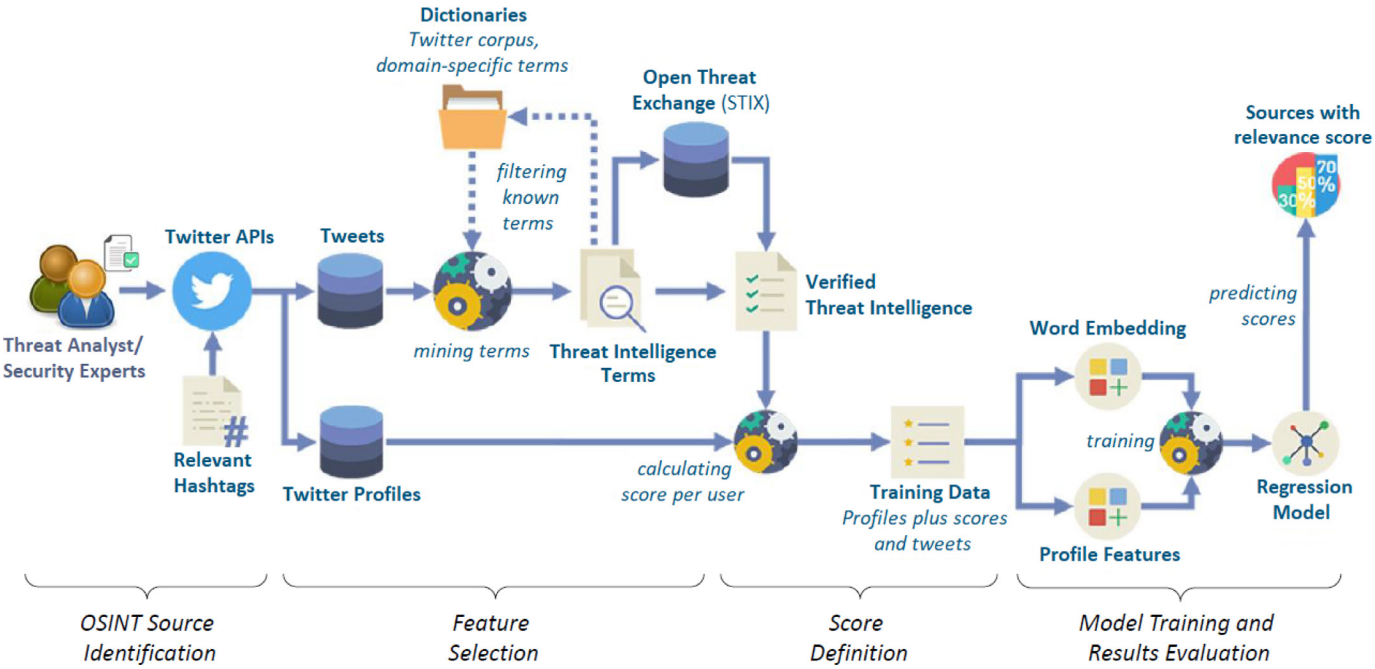
\includegraphics[width=1.0\linewidth]{images/research-method-overview.png}  % If located in the "images" folder
        \caption{Research method overview proposed by \citep{tundis2022feature}}
        \label{fig:thing1}
    \end{figure}
\end{itemize}


\paragraph{Analysis Medium}
\textit{Role and Functionality:} This component transforms raw data into actionable intelligence through pre-processing, correlation analysis, pattern detection, and anomaly recognition. The analysis medium uses algorithms and heuristics to classify and prioritize threats.

\textit{Literature Examples:}
\begin{itemize}
    \item \citep{kim2016know}: Emphasized the importance of structured data analysis, correlation techniques, and the use of YARA rules for malware detection. Their research shows how the analysis medium can derive meaningful insights from large datasets.
    \item \citep{noor2019machine}: Proposed an analysis approach that incorporates cyber threat attribution, helping organizations understand the origin and intent behind cyber-attacks.
    \item \citep{islam2022smartvalidator}: Integrated network data with a threat detector and alert validation system, highlighting the necessity of real-time data analysis to reduce false positives and improve threat response.
\end{itemize}

\paragraph{Information Platform}
\textit{Role and Functionality:} This component acts as the user interface and decision-support system for disseminating analyzed intelligence. It allows for threat information sharing, real-time monitoring, and supports collaborative efforts among stakeholders.

\textit{Literature Examples:}
\begin{itemize}
    \item \citep{bohm2018graph}: Designed a CTI information platform with features like data filtering, mapping, rendering, and user interaction. Their focus was on making threat intelligence more accessible and actionable for security teams.
    \item \citep{kim2016know}: Focused on the conversion of data into security rules, making the information platform a critical part of cybersecurity operations. This framework highlighted the use of automated security updates based on the analyzed intelligence.
    \item \citep{papastergiou2021handling}: Proposed a comprehensive information-sharing model that integrates deep and dark web mining, live monitoring, and data protection orchestrators. Their approach, which included the HybridNet and ShareNet components, emphasizes the importance of robust and secure information dissemination.
\end{itemize}

\subsection{Advanced Data Analytics and Machine Learning in CTI}
The application of advanced data analytics and machine learning in CTI frameworks \citet{naseer2023machine} is becoming increasingly prevalent. These technologies enhance the capability to detect patterns, classify threats, and predict future cyber-attacks.

\subsection*{Machine Learning Techniques}
Algorithms such as decision trees, support vector machines (SVMs) \citet{deliu2017extracting}, and neural networks \citet{yu2023tactics} are commonly used for threat detection. Unsupervised learning methods, like clustering, help in identifying unknown threat patterns, while supervised learning assists in classifying known threats.

\subsection*{Data Fusion and Anomaly Detection}
Techniques like time-series analysis and real-time data fusion \citet{song2022time} are essential for identifying anomalies in network behavior. For instance, \citet{islam2022smartvalidator} utilized data from both network and business operations to validate alerts and ensure that only genuine threats are flagged.

\subsection*{Case Studies in Industrial Settings}
Review studies that have successfully implemented machine learning in critical infrastructure protection, such as detecting anomalies in SCADA systems or preventing ransomware attacks. Discuss how these methods can be adapted to the mining industry.

\subsection*{Collaborative Cybersecurity Initiatives and Intelligence Sharing}
\begin{itemize}
    \item \textbf{Industry Partnerships and Alliances:} The role of collaborations among mining companies and cybersecurity organizations in improving threat intelligence capabilities.
    \item \textbf{Information Sharing Platforms:} The significance of platforms like ISACs (Information Sharing and Analysis Centers) that facilitate threat intelligence sharing across the industry.
    \item \textbf{Global Cybersecurity Alliances:} Participation in global threat intelligence networks to stay updated on emerging cross-border cyber threats.
\end{itemize}

\subsection*{Future Trends and Emerging Threats}
\begin{itemize}
    \item \textbf{Zero Trust Architecture \citet{stafford2020zero}:} Exploring the adoption of zero trust principles in securing industrial networks.
    \item \textbf{Blockchain Technology \citet{prakash2022blockchain}:} The potential of blockchain for securing data and communications in mining operations.
    \item \textbf{Quantum Computing Risks \citet{brooks2024inside}:} How advancements in quantum computing could pose new cybersecurity threats to the mining industry.
\end{itemize}

% Chapter 3
\chapter{Research Methodology}

\section{Research Design}

This research adopts a multi-phase design tailored to address the unique cybersecurity challenges encountered by the mining industry. The study is structured to incorporate both qualitative and quantitative approaches, integrating data from various sources and analyzing it through machine learning techniques to develop a specialized Cyber Threat Intelligence (CTI) framework. The research follows an iterative design that involves data collection, model development, ethical considerations, and system evaluation, as outlined in the following phases.

\subsection{Phase 1: Requirements Analysis and Literature Review}
The initial phase involves a comprehensive literature review and requirements analysis to understand the existing cybersecurity landscape within the mining industry. Key activities include:
\begin{itemize}
    \item \textbf{Stakeholder Engagement:} Conduct interviews and surveys with stakeholders, including cybersecurity professionals, to identify specific threats and security gaps in the mining sector.
    \item \textbf{Literature Review:} Examine existing CTI frameworks, cybersecurity models, and machine learning techniques relevant to critical infrastructure, particularly in industrial settings.
    \item \textbf{Gap Analysis:} Identify limitations in current CTI solutions and the specific needs of mining operations that require a tailored approach.
\end{itemize}

\subsection{Phase 2: Data Collection and Preprocessing}
This phase focuses on gathering and preparing data necessary for developing and testing the CTI framework. Key activities include:
\begin{itemize}
    \item \textbf{Data Sources:} Collect data from multiple sources, including network logs, OSINT (Open Source Intelligence) feeds, vendor-provided threat reports, and historical attack data in the mining industry.
    \item \textbf{Data Preprocessing:} Clean and transform the data to ensure quality and consistency. This involves handling missing values, normalizing data formats, and applying feature extraction techniques such as Principal Component Analysis (PCA) for noise reduction.
    \item \textbf{Data Labeling:} Label data samples with assistance from cybersecurity experts to distinguish between benign and malicious activities, enhancing model training accuracy.
\end{itemize}

\subsection{Phase 3: Framework Development and Modelling}
In this phase, the CTI framework’s architecture is designed and machine learning models are developed to detect, classify, and predict cyber threats in the mining sector. Key activities include:
\begin{itemize}
    \item \textbf{Framework Architecture Design:} Create an architecture blueprint that integrates data collection, preprocessing, analysis, and decision-support components of the CTI system.
    \item \textbf{Model Selection:} Select machine learning algorithms suitable for anomaly detection and threat classification, such as decision trees, support vector machines (SVM), or neural networks.
    \item \textbf{Model Training:} Train and validate models using supervised and unsupervised learning techniques on labeled data to maximize threat detection accuracy.
    \item \textbf{Feature Engineering:} Conduct feature engineering and exploratory data analysis to identify the most relevant indicators of cyber threats.
\end{itemize}

\subsection{Phase 4: System Evaluation and Optimization}
Once the CTI framework is developed, it undergoes rigorous testing and evaluation to ensure performance and reliability. Key activities include:
\begin{itemize}
    \item \textbf{Model Validation:} Validate the model’s performance on test datasets, evaluating metrics such as accuracy, precision, recall, and F1-score.
    \item \textbf{System Testing:} Conduct stress tests and simulate real-world threat scenarios in a controlled environment to evaluate the system’s responsiveness and robustness.
    \item \textbf{Hyperparameter Tuning:} Optimize model performance through hyperparameter tuning, such as grid search or random search, to enhance detection accuracy and reduce false positives.
    \item \textbf{Scalability Assessment:} Assess the framework’s scalability to ensure it can handle large volumes of data generated in mining operations.
\end{itemize}

\subsection{Phase 5: Ethical Considerations and Compliance}
This phase involves addressing the ethical and regulatory aspects of deploying a CTI system in the mining sector, focusing on data privacy and operational transparency. Key activities include:
\begin{itemize}
    \item \textbf{Privacy Safeguards:} Implement data anonymization and encryption techniques to protect sensitive information and ensure compliance with data protection regulations.
    \item \textbf{Bias and Fairness Analysis:} Regularly audit machine learning models to detect and mitigate biases, ensuring fair and accurate threat detection across various operational scenarios.
    \item \textbf{Ethics Approval:} Seek ethical approval from relevant bodies and consult industry experts to ensure that the framework aligns with both legal standards and industry guidelines.
\end{itemize}

\subsection{Phase 6: Documentation and Final Reporting}
The final phase documents the research findings and provides guidelines for practical implementation of the CTI framework in the mining industry. Key activities include:
\begin{itemize}
    \item \textbf{Results Documentation:} Summarize findings, including insights into CTI framework performance, challenges, and opportunities for improvement.
    \item \textbf{Recommendations for Implementation:} Provide recommendations for deploying the CTI framework in operational settings within the mining sector.
    \item \textbf{Final Report Preparation:} Compile and submit a comprehensive research report, detailing methodologies, results, and suggestions for future research directions.
\end{itemize}

This structured, multi-phase approach ensures a thorough and systematic investigation into the development of a CTI framework for the mining industry, addressing both technical and ethical considerations while aiming to contribute valuable insights to the field of cybersecurity in critical infrastructure.


\section{Methods}
The research will follow a comprehensive, multi-phase approach tailored to address the unique cybersecurity challenges encountered by the mining industry. The process will begin with a requirements analysis, which will involve collecting stakeholder opinions and reviewing relevant literature to identify specific needs and gaps in current cybersecurity frameworks. Then, during the framework development phase, a customized architecture will be developed, integrating data from various sources, such as network logs and open-source intelligence feeds. Following this, real-time threat data will be collected and aggregated, which will then be analyzed using advanced machine learning techniques to detect patterns, classify, and cluster the logs and anomalies. Ethical considerations will be carefully examined to ensure compliance with industry regulations and data privacy standards. A prototype of the CTI System will be developed and tested in a controlled environment to evaluate its effectiveness. Then, the system’s performance will be assessed, and detailed documentation will be prepared, offering insights and recommendations for practical implementation within the mining industry.

\subsection{Pre-Modelling Phase}
The pre-modelling phase focuses on the initial setup and preparation needed to build an effective Cyber Threat Intelligence (CTI) system. It includes data collection, data preprocessing, and defining the threat intelligence goals specific to the mining industry.

\begin{itemize}
    \item \textbf{Data Collection}: Raw data is collected from various sources such as network logs, open-source intelligence (OSINT) feeds, and vendor-specific threat intelligence reports. In mining operations, sensor and operational data can also be leveraged to detect abnormal patterns in the network.
    \item \textbf{Data Preprocessing}: The collected data is cleaned and transformed into a usable format. This involves handling missing data, removing duplicates, and normalizing data formats. Feature extraction techniques such as Principal Component Analysis (PCA) can be applied to reduce noise.
    \item \textbf{Data Labeling}: For supervised learning, historical data is labeled by domain experts as normal or malicious based on past incidents.
    \item \textbf{Goal Definition}: Specific objectives are defined, such as detecting ransomware, Advanced Persistent Threats (APTs), or insider threats, which will influence the models and algorithms chosen in the next phase.
\end{itemize}

\subsection{Modelling Phase}
The modelling phase involves building machine learning models that predict and detect cyber threats based on the pre-processed data.

\begin{itemize}
    \item \textbf{Model Selection}: Machine learning models such as decision trees, random forests, support vector machines (SVMs), or neural networks are selected based on the data type and threat scenarios.
    \item \textbf{Feature Engineering}: Relevant features are engineered to improve the model’s ability to detect cyber threats. Time-series analysis may be used for real-time threat detection in operational environments.
    \item \textbf{Model Training}: Models are trained using supervised learning on labeled data or unsupervised learning on unlabelled data to detect anomalies. Cross-validation techniques are used to avoid overfitting.
    \item \textbf{Threat Classification}: The trained model is used to classify network activity or system behavior into predefined threat categories (e.g., malware, phishing, Denial of Service attacks).
\end{itemize}

\subsubsection{Risk Assessment and Threat Probability}
The probability of a cyber threat occurring can be evaluated using Bayesian Probability or Conditional Probability models, which estimate threat likelihood given past occurrences or indicators.

\subsubsection{Bayesian Probability}
\[
P(A|B) = \frac{P(B|A) \cdot P(A)}{P(B)}
\]
Where:
\begin{itemize}
    \item \( P(A|B) \) is the probability of threat \( A \) given evidence \( B \).
    \item \( P(B|A) \) is the probability of evidence \( B \) given that threat \( A \) has occurred.
    \item \( P(A) \) is the prior probability of threat \( A \).
    \item \( P(B) \) is the total probability of evidence \( B \).
\end{itemize}

\subsubsection{Expected Risk (ER)}
\[
ER = P(T) \times C(T)
\]
Where:
\begin{itemize}
    \item \( P(T) \) is the probability of a specific threat occurring.
    \item \( C(T) \) is the cost impact of the threat.
\end{itemize}

\subsubsection{Anomaly Detection Using Statistical Analysis}
Anomalies in network behavior can indicate a possible cyber threat. Statistical techniques like mean and standard deviation are used to identify unusual behavior in a dataset.

\subsubsection{Mean (\(\mu\))}
\[
\mu = \frac{1}{N} \sum_{i=1}^N x_i
\]

\subsubsection{Standard Deviation (\(\sigma\))}
\[
\sigma = \sqrt{\frac{1}{N} \sum_{i=1}^N (x_i - \mu)^2}
\]

\subsubsection{Z-score for Anomaly Detection}
\[
Z = \frac{X - \mu}{\sigma}
\]
Where \( Z \)-score measures how far a data point \( X \) is from the mean in terms of standard deviations, which can help identify outliers or anomalies.

\subsubsection{Time Series Analysis for Anomaly Detection}
Time-series models in CTI are used to detect temporal patterns or changes in network behavior over time.

\subsubsection{Autoregressive Model (AR)}
\[
X_t = c + \phi_1 X_{t-1} + \phi_2 X_{t-2} + \dots + \phi_p X_{t-p} + \epsilon_t
\]
Where:
\begin{itemize}
    \item \( X_t \) is the value at time \( t \).
    \item \( \phi \) represents model parameters.
    \item \( \epsilon_t \) is white noise.
\end{itemize}

\subsubsection{Moving Average (MA) Model}
\[
X_t = \mu + \theta_1 \epsilon_{t-1} + \theta_2 \epsilon_{t-2} + \dots + \theta_q \epsilon_{t-q}
\]
Time-series modeling can help identify anomalies by looking for deviations from expected patterns.

\subsubsection{Game Theory in Threat Intelligence}
Game theory can model attacker-defender interactions, evaluating possible moves and responses in cybersecurity.

\subsubsection{Payoff Matrix}
Let \( A \) and \( D \) be attacker and defender strategies, respectively:
\[
\begin{array}{c|cc}
      & D_1 & D_2 \\
\hline
A_1 & P_{11} & P_{12} \\
A_2 & P_{21} & P_{22} \\
\end{array}
\]
Where:
\begin{itemize}
    \item \( P_{ij} \) represents the payoff for choosing strategy \( A_i \) against \( D_j \). Game theory helps in strategic planning and resource allocation for defense.
\end{itemize}

\subsubsection{Markov Chains for Threat Propagation Analysis}
Markov Chains model the likelihood of moving from one state (e.g., security level) to another, useful for understanding threat progression.

\subsubsection{Markov Chain Transition Probability}
\[
P(X_{t+1} = s_j | X_t = s_i) = p_{ij}
\]
Where \( p_{ij} \) is the probability of transitioning from state \( s_i \) to state \( s_j \). This method is useful for predicting future system states based on current security conditions.

\subsection{Post-Modelling Phase}
After building the models, the post-modelling phase focuses on evaluation, validation, and deployment.

\begin{itemize}
    \item \textbf{Model Validation}: Models are validated using test datasets. Key performance metrics such as accuracy, precision, recall, and F1 score are used to measure the model’s effectiveness.
    \item \textbf{Model Tuning}: Hyperparameter tuning (e.g., grid search or random search) is used to optimize the model. This process involves adjusting key parameters to improve performance.
    \item \textbf{Deployment Readiness}: Once validated, the model is integrated into existing systems (e.g., Security Information and Event Management systems) for real-time threat detection. The model undergoes stress testing to ensure it can handle real-time data streams.
\end{itemize}

\subsection{Experimental Setup}
The experimental setup defines how the CTI models are tested in a controlled environment before full deployment.

\begin{itemize}
    \item \textbf{Test Environment Setup}: A simulated or controlled mining network is created, including virtual machines, network traffic simulators, and log generators to mimic realistic scenarios.
    \item \textbf{Data Injection}: Historical data and simulated attack data are injected into the system to evaluate its ability to detect and respond to various threats.
    \item \textbf{Performance Measurement}: The system’s performance is measured using metrics such as detection rate, false alarm rate, and response time. Resource usage (CPU, memory) is also monitored to ensure scalability.
    \item \textbf{Comparison with Existing Systems}: The CTI framework’s performance is compared to existing cybersecurity systems in the mining industry to assess improvements.
\end{itemize}

\subsection{Optimization and Training Models}
The optimization and training phase focuses on refining the models to maximize their performance and efficiency.

\begin{itemize}
    \item \textbf{Hyperparameter Optimization}: Techniques such as grid search or Bayesian optimization are used to identify the best hyperparameters (e.g., learning rates, kernel functions) to improve detection accuracy.
    \item \textbf{Continuous Learning}: As new threats emerge, the model is retrained with updated data. Incremental learning or transfer learning methods may be used to update the model without complete retraining.
    \item \textbf{Efficiency Optimization}: The model is optimized for real-time performance through techniques such as model pruning, quantization, or the use of lightweight architectures.
    \item \textbf{Final Model Training}: The final optimized model is trained on the entire dataset to ensure robustness and accuracy. It is then ready for deployment into the CTI system.
\end{itemize}

\section{Limitations}

The primary limitation of this research is its reliance on a specific set of data sources and scenarios, which may restrict the generalizability of findings across the varied operational environments within the mining industry. Although the study aims to develop a comprehensive Cyber Threat Intelligence (CTI) framework tailored to mining, it is constructed on data samples and hypothetical scenarios that might not reflect all real-world conditions in diverse mining settings. Differences in operational practices, network architectures, and security postures across various geographical and organizational contexts could affect the performance and adaptability of the CTI framework. Additionally, the complexity and diversity of cyber threat data can lead to varying levels of success in detecting advanced threats, depending on the data quality and volume accessible in specific mining operations. Furthermore, this study may face challenges in replicating the full range of possible cyber-attack vectors in a controlled environment, which may limit the robustness of real-world application and implementation. Lastly, the scalability of the CTI system may be impacted by the computational resources required to process and analyze vast data sources, posing an additional limitation to the system’s practical deployment in certain resource-constrained mining operations.

\section{Ethical Considerations}

Ethical considerations are paramount in the design and implementation of a Cyber Threat Intelligence (CTI) framework, especially in a critical industry such as mining. One of the foremost concerns is ensuring data privacy and confidentiality, particularly in handling sensitive operational and employee-related data. Adherence to data protection regulations such as the General Data Protection Regulation (GDPR) and sector-specific cybersecurity regulations is essential to protect individual privacy and uphold legal standards. The CTI system’s capacity to monitor network traffic and detect anomalous behavior may inadvertently collect personally identifiable information (PII) or proprietary operational data, necessitating robust data anonymization and encryption measures.

Moreover, transparency and accountability in the use of machine learning algorithms for threat detection are critical to address biases or misclassifications that could lead to unintended consequences, such as falsely attributing benign activities as malicious or disproportionately scrutinizing certain behaviors. To mitigate such risks, regular audits and model validation steps are incorporated to maintain fairness and accuracy in detection algorithms. Additionally, ethical oversight will be applied to ensure that the CTI system does not lead to invasive surveillance or monitoring practices that infringe upon employees’ rights. Finally, collaboration with industry stakeholders and adherence to ethical guidelines ensure that the CTI framework is aligned with both industry standards and the ethical principles of autonomy, transparency, and justice in cybersecurity.

% % End of Chapter 3
\chapter{Schedule of Work}

This chapter outlines the schedule of work for the development of a Cyber Threat Intelligence (CTI) framework tailored to the mining industry. The research is planned over a 12-month period, starting from December 1, 2024, to November 30, 2025. Each phase consists of specific tasks aimed at meeting the objectives of this research.

\section{Overview}

The research schedule is divided into six phases: Initial Planning and Literature Review, Pre-Modelling and Data Preparation, Modelling and Machine Learning, System Evaluation and Optimization, Continuous Learning and Model Refinement, and Documentation and Final Reporting. Each phase addresses key tasks needed to develop, test, and validate a CTI framework designed for the unique cybersecurity needs of the mining industry.

\begin{longtable}{|p{4cm}|p{9.5cm}|p{2.5cm}|}
    \caption{Research Schedule from December 2024 to November 2025} \label{table:schedule_of_work} \\
    \hline
    \textbf{Phase} & \textbf{Activity Description} & \textbf{Timeline} \\
    \hline\hline
    \endfirsthead

    \hline
    \textbf{Phase} & \textbf{Activity Description} & \textbf{Timeline} \\
    \hline\hline
    \endhead

    \hline \multicolumn{3}{r}{\textit{Continued on next page}} \\
    \endfoot

    \hline
    \endlastfoot

    \textbf{Phase 1: Initial Planning and Literature Review} & & December 2024 - February 2025 \\
    \hline
    Requirements Analysis and Stakeholder Engagement & Conduct initial meetings with stakeholders to identify specific cybersecurity needs and define the project scope. & Dec 2024 - Jan 2025 \\
    \hline
    Literature Review & Review relevant literature on CTI frameworks, machine learning models, and cybersecurity within the mining sector to build a theoretical foundation. & Jan - Feb 2025 \\
    \hline
    Ethical and Regulatory Review & Review data privacy regulations and ethical standards for cybersecurity in mining to ensure compliance. & Feb 2025 \\
    \hline
    \textbf{Phase 2: Pre-Modelling and Data Preparation} & & March - April 2025 \\
    \hline
    Data Collection & Gather data from multiple sources, including network logs, OSINT feeds, and vendor-specific threat intelligence reports. & Mar 2025 \\
    \hline
    Data Preprocessing & Clean, transform, and normalize collected data, applying techniques such as PCA for noise reduction. & Mar - Apr 2025 \\
    \hline
    Goal Definition and Data Labeling & Define objectives for CTI (e.g., ransomware detection) and label historical data as normal or malicious based on prior incidents. & Apr 2025 \\
    \hline
    \textbf{Phase 3: Modelling and Machine Learning} & & May - July 2025 \\
    \hline
    Model Selection and Initial Testing & Choose initial machine learning models and test them on sample data to assess suitability for mining-specific cybersecurity needs. & May 2025 \\
    \hline
    Feature Engineering & Optimize feature sets for threat detection based on exploratory data analysis. & May - Jun 2025 \\
    \hline
    Model Training and Evaluation & Train models using supervised and unsupervised learning techniques, evaluating performance with metrics such as accuracy, precision, and recall. & Jun - Jul 2025 \\
    \hline
    Threat Classification & Classify network activity and system behavior into threat categories, such as malware or phishing attacks. & Jul 2025 \\
    \hline
    \textbf{Phase 4: System Evaluation and Optimization} & & August - September 2025 \\
    \hline
    Model Validation & Validate models using test datasets, fine-tuning hyperparameters to maximize performance. & Aug 2025 \\
    \hline
    Deployment Readiness & Prepare the validated model for deployment in a simulated mining environment and conduct stress testing. & Aug 2025 \\
    \hline
    Experimental Setup & Establish a controlled testing environment, including data injection and monitoring for system performance assessment. & Sep 2025 \\
    \hline
    \textbf{Phase 5: Continuous Learning and Model Refinement} & & October 2025 \\
    \hline
    Hyperparameter Optimization & Refine hyperparameters using techniques such as grid search or Bayesian optimization to improve model accuracy. & Oct 2025 \\
    \hline
    Continuous Learning & Implement incremental learning methods to keep the model updated with new data and emerging threats. & Oct 2025 \\
    \hline
    \textbf{Phase 6: Documentation and Final Reporting} & & November 2025 \\
    \hline
    Results Documentation & Summarize findings, including insights on CTI framework performance and areas for improvement. & Nov 2025 \\
    \hline
    Recommendations and Practical Implementation & Provide guidelines for practical implementation of the CTI framework in the mining industry. & Nov 2025 \\
    \hline
    Final Report Preparation & Compile and submit the final research report, detailing methodologies, results, and recommendations for future research. & Nov 2025 \\
\end{longtable}

\section{Detailed Timeline by Month}

\begin{itemize}
    \item \textbf{December 2024 - February 2025:} Requirements analysis, literature review, and ethical/regulatory assessment.
    \item \textbf{March - April 2025:} Data collection, preprocessing, and labeling for specific threat categories.
    \item \textbf{May - July 2025:} Selection, testing, and training of machine learning models, along with threat classification.
    \item \textbf{August - September 2025:} Model validation, deployment preparation, and experimental setup.
    \item \textbf{October 2025:} Hyperparameter optimization and continuous learning integration.
    \item \textbf{November 2025:} Documentation of findings, preparation of final report, and recommendations for implementation.
\end{itemize}


% This chapter outlines the schedule of work for the development of a Cyber Threat Intelligence (CTI) framework tailored to the mining industry. The research will take place over a 12-month period from December 1, 2024, to November 30, 2025. Each phase is allocated specific tasks to ensure timely progress and effective completion.

% \section{Overview}
% The research schedule is divided into several phases: Initial Planning and Literature Review, Pre-Modelling Data Preparation, Modelling and Machine Learning, System Evaluation and Optimization, and Documentation and Final Reporting. Each phase is structured to address the primary objectives of developing, testing, and validating a CTI framework designed for the unique cybersecurity needs of the mining industry.

% \section{Research Schedule}

% % \usepackage{pdflscape}
% % \usepackage{pdflscape}

% \begin{landscape}
% \begin{table}[p]
%     \centering
%     \caption{Research Schedule from December 2024 to November 2025}
%     \label{table:schedule_of_work}
%     \begin{tabular}{|p{4cm}|p{12cm}|p{3cm}|}
%         \hline
%         \textbf{Phase} & \textbf{Activity Description} & \textbf{Timeline} \\
%         \hline\hline
%         \textbf{Phase 1: Initial Planning and Literature Review} & & December 2024 - February 2025 \\
%         \hline
%         Requirements Analysis and Stakeholder Engagement & Conduct initial meetings with stakeholders to gather specific cybersecurity needs and define project scope. & Dec 2024 - Jan 2025 \\
%         \hline
%         Literature Review & Review relevant literature on CTI frameworks, machine learning models, and cybersecurity in the mining industry to establish a theoretical foundation. & Jan 2025 - Feb 2025 \\
%         \hline
%         Ethical and Regulatory Review & Review data privacy regulations and ethical guidelines relevant to cybersecurity in the mining industry. & Feb 2025 \\
%         \hline
%         \textbf{Phase 2: Pre-Modelling and Data Preparation} & & March - April 2025 \\
%         \hline
%         Data Collection & Collect data from various sources, including network logs, OSINT feeds, and threat intelligence reports. & Mar 2025 \\
%         \hline
%         Data Preprocessing & Clean, transform, and normalize data. Apply feature extraction techniques such as PCA for noise reduction. & Mar - Apr 2025 \\
%         \hline
%         Goal Definition and Data Labeling & Define specific objectives for CTI (e.g., ransomware detection) and label historical data as normal or malicious. & Apr 2025 \\
%         \hline
%         \textbf{Phase 3: Modelling and Machine Learning} & & May - July 2025 \\
%         \hline
%         Model Selection and Initial Testing & Select initial machine learning models and test them on sample data to determine suitability. & May 2025 \\
%         \hline
%         Feature Engineering & Refine and optimize feature sets based on exploratory data analysis. & May - Jun 2025 \\
%         \hline
%         Model Training and Evaluation & Train models using supervised and unsupervised learning on labeled data. Evaluate metrics such as accuracy, precision, and recall. & Jun - Jul 2025 \\
%         \hline
%         Threat Classification & Classify network activity or system behavior into specific threat categories, such as malware or phishing. & Jul 2025 \\
%         \hline
%         \textbf{Phase 4: Post-Modelling and System Evaluation} & & August - September 2025 \\
%         \hline
%         Model Validation & Validate models with test datasets, refining hyperparameters to optimize performance. & Aug 2025 \\
%         \hline
%         Deployment Readiness & Prepare the validated model for deployment in a simulated mining environment and conduct stress testing. & Aug 2025 \\
%         \hline
%         Experimental Setup & Define and set up a controlled environment, including test data injection and system monitoring. & Sep 2025 \\
%         \hline
%         \textbf{Phase 5: Optimization and Continuous Learning} & & October 2025 \\
%         \hline
%         Hyperparameter Optimization & Optimize hyperparameters using grid search or Bayesian optimization to improve model accuracy. & Oct 2025 \\
%         \hline
%         Continuous Learning & Implement mechanisms for incremental learning to update the model with new threat data. & Oct 2025 \\
%         \hline
%         \textbf{Phase 6: Documentation and Final Reporting} & & November 2025 \\
%         \hline
%         Results Documentation & Summarize findings, including insights on CTI framework performance and areas for improvement. & Nov 2025 \\
%         \hline
%         Recommendations and Practical Implementation & Provide guidelines and recommendations for deploying the CTI framework in the mining industry. & Nov 2025 \\
%         \hline
%         Final Report Preparation & Prepare and submit the final research report, including methodologies, results, and future directions. & Nov 2025 \\
%         \hline
%     \end{tabular} 
% \end{table}
% \end{landscape}

  
% Chapter 5
\chapter{Conclusion}
The CTI System for the Mining Industry aims to bridge the gap between the mining industry's unique operational demands and the growing need for robust cybersecurity measures. By developing a tailored CTI System, the study seeks to provide an architecture design of a CTI System. The development of the CTI System will enhance the ability to detect and respond to cyber threats proactively in the mining industry. The CTI System's integration of advanced data analytics and machine learning will offer more precise and real-time action against evolving threats. Additionally, this research will address ethical and regulatory concerns and ensure the proposed solution is effective and compliant with mining industry standards.
The findings from this research will contribute significantly to both the mining industry and the broader field of cybersecurity. By providing a specialized system for cyber threat intelligence, this study will help safeguard critical mining operations, protecting both assets and the environment. The lessons learned and the methodologies developed can serve as a model for other industries facing similar cybersecurity challenges, marking a step forward in the ongoing effort to secure vital industrial infrastructure.



% \LaTeX\ decides how to place images. It also does the referencing for you as seen in \Cref{fig:thing1}. If you have subimages, they should have their own captions and labels -- look into the subfig or subfigure packages.

% Including the image with correct file extension


% Figure captions are at the bottom. Table titles are at the top of the table as seen in \Vref{tab:tab1}. 

% \begin{table}[p]
%   \centering
%   \caption{Table Name}
%   \label{tab:tab1}
%   \begin{tabular}{cc}
%       \hline
%       Col1 & Col2\\
%       \hline\hline 
%       R0,C0 & R0,C1 \\ 
%       R1,C0 & R1,C1 \\ 
%       \hline
%   \end{tabular} 
% \end{table}

% \chapter{Some Referencing Tricks}
% CleverRef and VarioRef are helpful:
% \begin{itemize}
%   \item Normal Ref: See Figure \ref{fig:thing1}
%   \item CleverRef: See \Cref{fig:thing1} and \Cref{tab:tab1}
%   \item CleverRef+VarioRef: See \Vref{fig:thing1} and \Vref{tab:tab1}
% \end{itemize}

% \chapter{IDE/Editors}
% Overleaf has a great online editor for latex. Use it. 

\appendix
\chapter{Extra Stuff}\label{app:extra}
\section{What is an appendix?}\label{app:whatis}

An appendix is useful when there is information that you need to include, but breaks the flow of your document, e.g. a large number of figures/tables may need to be shown, but maybe only one needs to be in the text and the rest are just included for completeness.

\nocite{*}


\bibliography{references}\addcontentsline{toc}{chapter}{References}
\end{document}


